\documentclass[aps,prd,twocolumn,superscriptaddress,nofootinbib,longbibliography]{revtex4-2}

\usepackage[utf8]{inputenc}
\usepackage[T1]{fontenc}
\usepackage{amsmath,amssymb,bm}
\usepackage{mathrsfs}
\usepackage{graphicx}
\usepackage{booktabs}
\usepackage{array}
\usepackage[colorlinks=true,linkcolor=blue,citecolor=blue,urlcolor=blue]{hyperref}

\newcommand{\dd}{\mathrm{d}}
\newcommand{\Lag}{\mathcal{L}}
\newcommand{\LD}{\mathfrak{L}}
\newcommand{\calS}{\mathcal{S}}
\newcommand{\calC}{\mathcal{C}}
\newcommand{\calD}{\mathcal{D}}
\newcommand{\Mp}{M_{\rm p}}
\newcommand{\Lam}{\Lambda}
\newcommand{\LCDM}{\Lambda{\rm CDM}}
\newcommand{\DES}{\mathrm{DES}}
\newcommand{\DESI}{\mathrm{DESI}}
\newcommand{\SN}{\mathrm{SN}}
\newcommand{\BAO}{\mathrm{BAO}}
\newcommand{\varphione}{\varphi_1}
\newcommand{\varphitwo}{\varphi_2}
\newcommand{\chiT}{\chi^2_{\rm tot}}

\begin{document}

\preprint{AI-MG-agent-benchmark-v1}

\title{Dark Energy Autonomous Search from Cosmological Background Data}

\author{Cooper Niu}
\affiliation{Department of Physics, Brown University, Providence, Rhode Island 02912, USA}

\author{Wenrong Sun}
\affiliation{Department of Physics, Brown University, Providence, Rhode Island 02912, USA}

\date{\today}


\begin{abstract}
We present a physics-first framework for the autonomous discovery of two-scalar modified-gravity backgrounds from late-time cosmological data.  Candidate theories are generated as covariant, dimension-balanced Lagrangian densities built from curvature tensors, covariant derivatives, and two scalar fields.  They are then subjected to deterministic physical validation: the FLRW equations are derived symbolically; algebraic coefficient relations are imposed at the equation-of-motion level to cancel all independent third- and higher-time derivatives in the gauge-fixed background equations; the lapse equation is retained as a modified Friedmann constraint; and the surviving systems are integrated and compared with DES type-Ia supernova distances and DESI Data Release 2 baryon-acoustic-oscillation measurements.  The artificial-intelligence component is used only to navigate the large discrete theory space and propose parameter samples; theoretical consistency and empirical scoring are decided by the physics pipeline.  The derivative-order filter should be read as a necessary FLRW Ostrogradsky-cancellation condition, not as a sufficient proof of full covariant ghost freedom.  We emphasize the role of temporal diffeomorphism invariance in the minisuperspace theory: even when a raw modified-gravity Lagrangian contains derivatives of the lapse before simplification, the residual time-reparametrization Noether identity implies that, on an FLRW branch whose dynamical equations have passed the cancellation filter, the gauge-fixed lapse equation is a first-order constraint rather than an independent dynamical equation, and this constraint is preserved by the evolution equations.  The representative v5.2.2-agent validations reported here find background solutions with $\chiT\simeq 1638$ for DES-SN plus DESI-DR2 BAO.  The best families are typically Einstein--Hilbert anchored scalar sectors, while a subset contains weak, moderate, or active curvature corrections.  These results identify promising background branches, not final fully viable gravitational theories; perturbation stability, structure growth, gravitational-wave constraints, and local tests remain necessary validation layers.
\end{abstract}

\maketitle

\section{Introduction}
\label{sec:introduction}

The observed acceleration of the Universe is one of the clearest indications that either the cosmic energy budget or the gravitational sector is not yet fully understood. The minimal $\Lambda$CDM model gives an effective description of current background data, but it treats the observed value of $\Lambda$ as an input parameter rather than explaining its smallness, origin, or late-time dominance. Modified gravity and scalar-tensor theories provide a systematic way to test whether late-time acceleration can arise from additional gravitational degrees of freedom rather than from a rigid vacuum energy \cite{Clifton2012,SotiriouFaraoni2010,Horndeski1974}.

The difficulty is not the absence of possible theories. It is the opposite: the space of covariant Lagrangians built from curvature invariants, derivatives, and scalar fields is combinatorially large.  Most expressions are physically unacceptable. Generic higher-derivative theories contain Ostrogradsky's instabilities \cite{Ostrogradsky1850}; many theories fail to admit a regular cosmological initial-value problem; and many stable background branches do not fit the data. Historically, theorists have navigated this landscape with symmetry, naturalness, simplicity, and experience. These principles remain essential, but they are incomplete search strategies in a high-dimensional theory space.

Recent DES supernova and DESI baryon-acoustic-oscillation measurements provide a sharp background-expansion target for such searches \cite{DES2024SN,DESI2025BAO}.  At the same time, recent work on autonomous theory discovery has shown that physics can be encoded as a formal language, so that artificial intelligence proposes only well-formed theories while deterministic computations impose first-principle constraints and evaluate data likelihoods \cite{Alexander2026Albert}.  We adopt a similar philosophy for modified gravity. The agent is not asked to hallucinate equations or to judge its own success. It proposes covariant operator combinations and numerical samples inside a fixed grammar. The theory is then accepted or rejected by an explicit symbolic and numerical pipeline.

This paper describes the physical content of the agent modified-gravity framework. The emphasis is deliberately different from a software manual.  The implementation details are documented in the public code; here we focus on the theory space, the FLRW derivative-order cancellation reduction, the modified Friedmann constraint, the construction of a dimensionless cosmological initial-value problem, and the interpretation of the resulting DES-SN and DESI-DR2 BAO fits.

\section{Covariant Theory Space}
\label{sec:theory-space}

\subsection{Dimension-balanced effective Lagrangians}
\label{subsec:dimension-balanced}

We consider a broad EFT-like space of metric theories containing two scalar fields, $\phi_1$ and $\phi_2$, with different characteristic scales.  A generated theory is stored and validated as a Lagrangian density,
\begin{equation}
\calS=\int \dd^4x\,\mathscr{L},
\qquad
\mathscr{L}=\sqrt{-g}\,\Lag ,
\label{eq:action}
\end{equation}
with the scalar bracket
\begin{equation}
\Lag=
\Mp^2\sum_{I\in G\cup N}
c_I\Lam^{2-d_I}O_I
+
\sum_{J\in S}c_J\Lam^{4-d_J}S_J
+
\Lag_{\rm fixed}.
\label{eq:lagrangian}
\end{equation}
Here $G$ denotes pure-curvature invariants, $N$ non-minimal scalar-curvature invariants, and $S$ pure-scalar generated invariants.  The integer $d_I$ is the mass dimension of the corresponding covariant scalar.  The factors of $\Mp^2$ and $\Lam$ ensure that each term in the density $\mathscr{L}$ has the correct mass dimension.  Thus a candidate is not specified by an operator label alone; its sector, coefficient, cutoff power, Planck-mass prefactor, fixed scalar matter terms, and outer $\sqrt{-g}$ are part of the physical theory.

The candidate building blocks include
\begin{equation}
R,\qquad R_{\mu\nu},\qquad R^\rho{}_{\sigma\mu\nu},\qquad
\nabla_\mu,\qquad \phi_1,\qquad \phi_2 .
\end{equation}
Examples of generated invariants are
\begin{equation}
R^2,\qquad
R_{\mu\nu}R^{\mu\nu},\qquad
\phi_1^2R,\qquad
\nabla_\mu\phi_1\nabla_\nu\phi_1R^{\mu\nu},\qquad
\Box\phi_1\,R.
\end{equation}
Up to mass dimension six, there are 141 independent curvature invariants on the FLRW background.
The scalar configurations are 
\begin{equation}
\hbox{none},\qquad \phi_1\hbox{ only},\qquad \phi_2\hbox{ only},\qquad \phi_1\text{ and }\phi_2 .
\end{equation}
When a scalar is active, the fixed matter sector contains a canonical kinetic term and either a quadratic or an axion-like potential:
\begin{align}
\Lag_{\rm fixed}^{(i)}
&=-\frac12 g^{\mu\nu}\nabla_\mu\phi_i\nabla_\nu\phi_i - V_i(\phi_i),\\
V_i(\phi_i)
&=\frac12 m_i^2\phi_i^2
\quad{\rm or}\quad
m_i^2f_i^2\left[1-\cos\left(\frac{\phi_i}{f_i}\right)\right].
\label{eq:fixed-sector}
\end{align}


The two scalar fields play different roles in the current theory grammar.  The first scalar is naturally measured in Planck units,
\begin{equation}
\phi_1=\Mp\varphione,
\end{equation}
while the second is measured in cutoff units,
\begin{equation}
\phi_2=\Lam\varphitwo .
\end{equation}
This hierarchy allows the search to include both Planck-normalized scalar-tensor sectors and cutoff-normalized EFT scalar structures.  The distinction matters because a term such as $\phi_2 R$ carries a different scale from $\phi_1 R$, even when their dimensionless field amplitudes are comparable.  It is therefore useful to parameterize the EFT cutoff in units of the present Hubble scale,
\begin{equation}
\lambda_H\equiv\frac{\Lam}{H_0}.
\label{eq:lambdaH}
\end{equation}
With $h\equiv H/H_0$, the dimensionless ratio between the background expansion scale and the cutoff is simply $H/\Lam=h/\lambda_H$.  This quantity enters the validation-stage scale-separation cut introduced in Sec.~\ref{sec:ivp}.

\section{Mini-Superspace and Background Physical Filtering}
\label{sec:ghost}

\subsection{Background equations}
\label{subsec:background-eom}

The first physical filter is applied after reducing the covariant theory on the spatially flat FLRW metric
\begin{equation}
\dd s^2=-N(t)^2\dd t^2+a(t)^2\delta_{ij}\dd x^i\dd x^j .
\label{eq:flrw}
\end{equation}
The minisuperspace variation gives
\begin{equation}
\delta S=\int \dd t\left(E_N\delta N+E_a\delta a+\sum_iE_{\phi_i}\delta\phi_i\right),
\label{eq:variation}
\end{equation}
where the inactive scalar equations are omitted.  After variation, the equations are evaluated in cosmic-time gauge, $N=1$:
\begin{equation}
E_N=0,\qquad E_a=0,\qquad E_{\phi_i}=0 .
\label{eq:eom-set}
\end{equation}
The lapse equation is not discarded.  It is the modified Friedmann equation, while $E_a$ and $E_{\phi_i}$ determine the dynamical evolution.


\subsection{Ostrogradsky ghost and FLRW cancellation relations}
\label{subsec:ostro}

Higher-curvature and derivative scalar-curvature operators generically produce equations containing third or higher time derivatives of $a(t)$ and $\phi_i(t)$.  If such derivatives represent independent initial data, the theory contains an Ostrogradsky mode: the Hamiltonian is unbounded and the background branch is a physically unacceptable ghost\cite{Ostrogradsky1850}.  The pipeline therefore treats the derivative order of the FLRW equations as a hard physical constraint before any likelihood evaluation.

The raw proposal grammar is deliberately broader than the standard Horndeski basis.  It can contain operators such as $R^2$, $R^3$, $\nabla R\nabla R$, or mixed scalar-curvature contractions.  These monomials should not be read as arbitrary higher-derivative theories after acceptance.  The EOM stage first derives the gauge-fixed FLRW equations and expands their forbidden higher-derivative part schematically as
\begin{equation}
E_A=E_A^{\leq 2}+
\sum_{B}\sum_{r\geq 3}{\cal A}_{AB}^{(r)}(a,\dot a,\phi_i,\dot\phi_i;c_I)
\,y_B^{(r)},
\label{eq:forbidden-derivatives}
\end{equation}
where $A$ labels the lapse, scale-factor, and active-scalar equations, $y_B\in\{a,\phi_i\}$, and the ${\cal A}_{AB}^{(r)}$ are algebraic functions of the operator coefficients and lower-derivative variables.  The background cancellation filter solves the coefficient constraints
\begin{equation}
{\cal A}_{AB}^{(r)}=0
\qquad
\hbox{for all independent }B\hbox{ and }r\geq 3,
\label{eq:cancellation-relations}
\end{equation}
and substitutes the resulting branch relations before passing the model to the Builder and Solver.  A model may therefore contain a displayed $R^2$, $R^3$, or derivative-curvature operator only as part of a coefficient-restricted FLRW-degenerate combination.  If the required relations force the relevant correction to zero, the model is interpreted as the corresponding lower-complexity branch rather than as evidence for an active higher-curvature correction.

This condition is Horndeski/DHOST-like in spirit, because it removes the would-be Ostrogradsky data by degeneracy rather than by assuming small higher derivatives \cite{Horndeski1974,Langlois2016DHOST}.  It is not identical to imposing the full covariant Horndeski Lagrangian at the proposal stage.  The proposal space is broader, while the acceptance condition is narrower and equation-level: the accepted branch must have FLRW equations with no independent third- or higher-time derivatives after the coefficient relations are imposed.

\subsection{The modified Friedmann constraint}
\label{sec:hamiltonian}
\label{subsec:modified-friedmann}



In ordinary GR, the FLRW lapse $N$ appears without time derivatives after the Einstein--Hilbert boundary term is handled.  The momentum conjugate to $N$ vanishes, and preserving this primary constraint gives the Hamiltonian constraint, which reduces to the Friedmann equation.  In a raw modified-gravity minisuperspace Lagrangian, however, $N$ may appear with derivatives before integrations by parts or before imposing the background derivative-cancellation relations.  Therefore the simple GR statement ``the lapse is a Lagrange multiplier'' is not always the cleanest way to identify the constraint.

The more robust argument comes from residual time-reparametrization invariance.  Under
\begin{equation}
t\rightarrow t-\xi(t),
\end{equation}
the minisuperspace variables transform as
\begin{equation}
\delta_\xi a=\xi\dot a,\qquad
\delta_\xi\phi_i=\xi\dot\phi_i,\qquad
\delta_\xi N=(N\xi)^{\cdot}.
\label{eq:time-diffeo}
\end{equation}
Invariance of the action under this transformation gives the off-shell Noether identity
\begin{equation}
N\dot E_N-\dot a\,E_a-\sum_i\dot\phi_i\,E_{\phi_i}=0.
\label{eq:noether}
\end{equation}
This is the minisuperspace form of the Bianchi identity.  It holds before imposing the equations of motion.



After gauge fixing to $N=1$, Eq.~\eqref{eq:noether} becomes
\begin{equation}
\dot E_N=\dot a\,E_a+\sum_i\dot\phi_i\,E_{\phi_i}.
\label{eq:noether-gauge}
\end{equation}
Suppose the background derivative-cancellation relations have made the dynamical equations $E_a=0$ and $E_{\phi_i}=0$ at most second order in time derivatives.  Then the right-hand side of Eq.~\eqref{eq:noether-gauge} contains no independent third derivatives.

If the gauge-fixed lapse equation $E_N|_{N=1}$ contained an acceleration, schematically
\begin{equation}
E_N|_{N=1}=C(a,\dot a,\ddot a,\phi_i,\dot\phi_i,\ddot\phi_i),
\end{equation}
then its time derivative would contain independent third derivatives:
\begin{equation}
\dot E_N|_{N=1}
\supset
\frac{\partial C}{\partial \ddot a}a^{(3)}
+\sum_i
\frac{\partial C}{\partial \ddot\phi_i}\phi_i^{(3)}.
\end{equation}
These terms cannot be matched by the right-hand side of Eq.~\eqref{eq:noether-gauge}.  Since the identity is off shell and holds for arbitrary field profiles, the coefficients of all independent third derivatives must vanish.  Therefore
\begin{equation}
E_N|_{N=1}=C_N(a,\dot a,\phi_i,\dot\phi_i),
\label{eq:first-order-constraint}
\end{equation}
and the lapse equation is a first-order constraint on FLRW initial data, not an independent second-order dynamical equation.


The same identity guarantees propagation of the constraint.  On solutions of the dynamical equations,
\begin{equation}
E_a=0,\qquad E_{\phi_i}=0,
\end{equation}
Eq.~\eqref{eq:noether-gauge} implies
\begin{equation}
\dot E_N=0.
\end{equation}
Thus if the initial data satisfy
\begin{equation}
E_N(t_0)=0,
\end{equation}
then the background evolution preserves
\begin{equation}
E_N(t)=0.
\end{equation}
This justifies using the lapse equation to solve for one initial velocity and then monitoring the residual constraint throughout numerical integration.

The result is deliberately limited to the background construction: within the FLRW derivative-cancelled sector, the lapse equation is a first-order modified Friedmann constraint, and the dynamical equations preserve it once it is imposed on the initial data.  The wider domain of validity of this minisuperspace statement is summarized next.

\subsection{Scope of the background filter}
\label{subsec:ghost-scope}

The preceding analysis imposes two distinct background-level requirements.  First, Eq.~\eqref{eq:cancellation-relations} removes all independent third- and higher-time derivatives from the gauge-fixed FLRW equations.  Second, the residual time-reparametrization identity makes the lapse equation a preserved first-order constraint on the accepted branch.  Together these conditions are necessary for the background initial-value problem, but they are not a sufficient proof of full covariant ghost freedom.  They do not establish the complete ADM/Dirac constraint algebra, the quadratic action for scalar and tensor perturbations, the sign of the kinetic matrix, gradient stability, the tensor propagation speed, or stability on non-FLRW backgrounds.  These checks are logically separate from the background search.  In this paper, ``accepted'' means that a branch has passed the FLRW derivative-order filter, admits a regular background initial-value problem, preserves the modified Friedmann constraint numerically, satisfies the stated background EFT cut, and yields a finite DES-SN plus DESI-DR2 BAO score.  It does not mean that the theory is already a fully viable modified-gravity model.

On this restricted background sector, the modified Friedmann constraint can be used to select initial data and the remaining equations can be cast as the dimensionless first-order system constructed next.

\section{Dimensionless Cosmological Initial-Value Problem}
\label{sec:ivp}

The numerical evolution uses e-fold time
\begin{equation}
x=\ln a=-\ln(1+z),
\qquad
h=\frac{H}{H_0},
\label{eq:xh}
\end{equation}
so that
\begin{equation}
\frac{\dd}{\dd t}=H_0h\frac{\dd}{\dd x}.
\label{eq:chain-rule}
\end{equation}
The relevant substitutions include
\begin{align}
\dot a&=H_0e^xh,
&
\ddot a&=H_0^2e^x(h^2+hh_x),\\
\dot\phi_1&=\Mp H_0h q_1,
&
\ddot\phi_1&=\Mp H_0^2h(h_xq_1+hq_{1x}),\\
\dot\phi_2&=H_0^2\lambda_H h q_2,
&
\ddot\phi_2&=H_0^3\lambda_H h(h_xq_2+hq_{2x}),
\label{eq:rescalings}
\end{align}
where
\begin{equation}
q_i=\frac{\dd\varphi_i}{\dd x}.
\end{equation}
Masses and decay constants are written as
\begin{equation}
m_1=H_0\mu_1,\qquad
m_2=\Lam\mu_2,\qquad
f_1=\Mp \bar f_1,\qquad
f_2=\Lam \bar f_2 .
\end{equation}

After these substitutions, the Builder forms dimensionless equations
\begin{equation}
C_N=0,\qquad C_a=0,\qquad C_{\phi_i}=0.
\end{equation}
The constraint $C_N=0$ is imposed at $x=0$ with $h(0)=1$.  The dynamical equations are solved algebraically for the highest e-fold derivatives,
\begin{equation}
\bm u=(h_x,q_{1x},q_{2x})^T.
\end{equation}
When a regular branch exists, the result is an explicit first-order system,
\begin{equation}
\frac{\dd}{\dd x}
\begin{pmatrix}
h\\ \varphione\\ q_1\\ \varphitwo\\ q_2
\end{pmatrix}
=
\begin{pmatrix}
F_h\\ q_1\\ F_1\\ q_2\\ F_2
\end{pmatrix},
\label{eq:first-order}
\end{equation}
with absent scalar variables omitted.  The trajectory is rejected if the constraint drifts beyond the production tolerance,
\begin{equation}
\max_x|C_N(x)|>10^{-4}.
\label{eq:constraint-cut}
\end{equation}
It is also rejected if the background expansion scale approaches the cutoff.  The validation-stage scale-separation cut is
\begin{equation}
\epsilon_H\equiv
\max_x\frac{|H(x)|}{\Lam}
=
\max_x\frac{|h(x)|}{\lambda_H}
<0.1 .
\label{eq:eft-cut}
\end{equation}
This is a hard background-level rejection criterion.  It ensures that the accepted trajectory remains below the cutoff scale probed by the homogeneous expansion, but it should not be read as a complete proof that the full EFT expansion is controlled.  The stronger field-excursion, kinetic, and operator-hierarchy diagnostics are discussed in Sec.~\ref{subsec:eft-diagnostics}.

\section{Cosmological Observables}
\label{sec:observables}

Each accepted solution gives a Hubble history $H(z)=H_0h(z)$.  The supernova distance modulus is computed from
\begin{equation}
D_L(z)=(1+z_{\rm hel})\frac{c}{H_0}
\int_0^{z_{\rm HD}}\frac{\dd z'}{h(z')},
\label{eq:luminosity-distance}
\end{equation}
with an analytically profiled absolute-magnitude offset.  The supernova likelihood therefore mainly constrains the relative shape of the distance-redshift relation.

The BAO observables are computed from the same background solution:
\begin{align}
\calD_M(z)&=\int_0^z\frac{\dd z'}{h(z')},\\
\calD_H(z)&=\frac{1}{h(z)},\\
\calD_V(z)&=\left[\frac{z\calD_M(z)^2}{h(z)}\right]^{1/3}.
\label{eq:bao}
\end{align}
In this background-only analysis, the BAO scale is profiled as a nuisance parameter.  Thus the DESI comparison should be interpreted as a relative-distance test of the late-time expansion history, not as a complete early-universe calculation of the sound horizon in each modified-gravity theory.

The primary score is
\begin{equation}
\chiT=\chi^2_{\DES\text{-}\SN}+\chi^2_{\DESI\text{-DR2}\,\BAO}.
\label{eq:chi2}
\end{equation}
Models are ranked by $\chiT$, with information criteria recorded only as secondary diagnostics \cite{Akaike1974,Schwarz1978}.

\section{Autonomous Search Strategy}
\label{sec:search}

The autonomous component follows the same principle as formal-language approaches to particle-physics discovery: generate theories inside a grammar, enforce hard theoretical constraints, compute observables with deterministic code, and reward agreement with data \cite{Alexander2026Albert}.  In the present work the grammar is a modified-gravity Lagrangian grammar rather than a particle-physics gauge grammar.  The hard constraints are covariance of the generated operators, dimension balancing, EOM-level FLRW ghost-cancellation relations, existence of a regular IVP, Friedmann-constraint preservation, and background EFT scale separation.  The empirical reward is the Solver-written $\chiT$.  Operationally, a proposal is compiled into isolated Lagrangian and parameter-sample files and then passed through the EOM, Builder, and Solver stages; the agent proposes, but the deterministic pipeline validates and scores.

The important point is that the search policy is not part of the physics claim.  Different proposal policies can explore the same theory space.  A candidate becomes physically interesting only when it passes the deterministic validation chain and produces an accepted cosmological trajectory.  For that reason we report accepted theories by their complete Lagrangian densities, coefficient values, scalar initial conditions, constraint residuals, and data-fit metrics rather than by agent prompts or internal training details.

The search has two coupled components: a discrete proposal over scalar content and covariant operator structure, and a continuous proposal over parameters and initial data.  We describe the structural sector allocation first and the continuous scan priors second.

\subsection{Proposal sectors and diagnostic comparisons}
\label{subsec:sector-separated-search}

To make the search output easier to interpret, mini-batch runs can separate proposal memory by sector while keeping the same deterministic validation pipeline.  The default sector split in the proposal schema contains an open-search sector and a non-EH sector.  The open-search sector samples the full grammar subject to the universal legality, FLRW ghost-cancellation, IVP, constraint, EFT, and likelihood filters.  The non-EH sector forbids the bare Einstein--Hilbert $R$ anchor and searches curvature or scalar-curvature theories that must compete without an explicit $\Mp^2R/2$ term.  In this default setting the proposal budget is
\begin{equation}
N_{\rm open}:N_{\rm non\text{-}EH}=1:1 .
\label{eq:default-sector-budget}
\end{equation}

For interpretability, some diagnostic runs add a third constrained lane that forces an Einstein--Hilbert anchor together with a $\phi_2$-only scalar configuration and at least one explicit $\phi_2$--curvature operator.  This lane isolates cutoff-normalized $\phi_2$ new-physics candidates from the easier Planck-normalized $\phi_1$ sector, but it is not the default sector in the proposal schema.  When such a triad diagnostic is quoted below, it should be read as a controlled discovery comparison with
\begin{equation}
N_{\rm open}:N_{\rm EH+\phi_2}:N_{\rm non\text{-}EH}=1:1:1,
\label{eq:triad-budget}
\end{equation}
not as a posterior probability over theory classes.

Each sector writes its own attempt history, failure tags, accepted-sample statistics, and best-per-family report.  The sector comparison is therefore a discovery diagnostic answering which branches the stated search policy can find efficiently under fixed budgets; it is not a Bayesian evidence calculation and it does not count FLRW-equivalent operator representatives as independent physical theories.


\subsection{Proposal parameters and scan ranges}
\label{subsec:parameter-priors}

Table~\ref{tab:parameter-priors} summarizes the default cold-start ranges for the continuous component of the search.  They are exploration priors rather than physical acceptance conditions: a sample drawn from these ranges is still rejected if it fails the modified Friedmann constraint, violates the background EFT cut, produces an irregular trajectory, or admits no acceptable real root for the constrained initial velocity.

\begin{table*}[t]
\centering
\begin{ruledtabular}
\begin{tabular}{lllll}
Parameter & Dimensionless definition & Applies to & Default range & Sampling scale \\
\hline
$H_0$ & $H_0\,[{\rm km\,s^{-1}\,Mpc^{-1}}]$ & all sectors & $58$--$74$ & linear \\
$\Omega_{m0}$ & $\rho_{m0}/(3\Mp^2H_0^2)$ & all sectors & $0.22$--$0.40$ & linear \\
$\lambda_H$ & $\Lam/H_0$ & all sectors & $5.0\times10^2$--$8.0\times10^4$ & log \\
$\varphi_{1,0}$ & $\phi_1(t_0)/\Mp$ & $\phi_1$ sectors & $10^{-3}$--$10^{1}$ & log \\
$\mu_1$ & $m_1/H_0$ & $\phi_1$ sectors & $10^{-2}$--$10^{2}$ & log \\
$\bar f_1$ & $f_1/\Mp$ & $\phi_1$ axion sectors & $10^{-2}$--$10^{2}$ & log \\
$\varphi_{2,0}$ & $\phi_2(t_0)/\Lam$ & $\phi_2$ sectors & $10^{-5}$--$10^{5}$ in $|\varphi_{2,0}|$ & signed log \\
$q_{2,0}$ & $\dd\varphi_2/\dd\ln a|_{0}$ & two-scalar sectors & $10^{-5}$--$10^{5}$ in $|q_{2,0}|$ & signed log \\
$\mu_2$ & $m_2/\Lam$ & $\phi_2$ sectors & $10^{-5}$--$10^{5}$ & log \\
$\bar f_2$ & $f_2/\Lam$ & $\phi_2$ axion sectors & $10^{-5}$--$10^{5}$ & log \\
$c_I$ & non-EH operator coefficients & generated operators & $10^{-10}$--$10^{20}$ in $|c_I|$ & log, both signs \\
\end{tabular}
\end{ruledtabular}
\caption{Default continuous proposal ranges.  These are broad cold-start exploration priors, not physical acceptance cuts.  The Einstein--Hilbert coefficient is not scanned: when the plain $R$ anchor is present it is fixed to $c_R=1/2$.  In one-scalar models the initial scalar velocity is solved from the modified Friedmann constraint rather than independently sampled.  In two-scalar models $q_{2,0}$ is sampled and the constraint solves for the remaining scalar velocity.  Signed-log sampling means that the sign is sampled separately and the listed range applies to the absolute value.}
\label{tab:parameter-priors}
\end{table*}

For higher-dimension curvature corrections, a naive coefficient prior can render the correction effectively invisible because of the associated powers of $\Lam$.  The scans therefore record an effective-size diagnostic and, in selected proposal modes, choose coefficient magnitudes that target weak, moderate, or active fractional corrections relative to the Einstein--Hilbert term.  We estimate
\begin{equation}
\Delta_i\simeq
\left|\frac{c_i}{c_{\rm EH}}\right|\lambda_H^{p_i}{\cal F}_i ,
\label{eq:delta-prior}
\end{equation}
where $p_i$ is the net power of $\lambda_H$ inherited from the dimension-balanced operator and ${\cal F}_i$ denotes the relevant dimensionless field factor.  The weak, moderate, and active-probe target intervals are approximately $10^{-6}$--$10^{-4}$, $10^{-4}$--$10^{-2}$, and $10^{-2}$--$10^{2}$, respectively.

The continuous sampler uses a 50/50 hybrid proposal policy: half of the samples are deterministic agent-exact anchors and half are stochastic draws.  Both branches may use the current-loop joint parameter memory, with a default usage fraction of $0.80$, by reusing or perturbing high-reward parameter vectors when available and otherwise reverting to the learned or default priors.  For non-EH curvature corrections, only the weak, moderate, and active-probe modes use the relative-effect prescription in Eq.~\eqref{eq:delta-prior}; the baseline mode instead samples raw signed-log coefficients from the broad prior.  These choices affect only the proposal distribution.  Physical acceptance and final ranking remain determined by the deterministic validation chain and the Solver value of $\chi^2_{\rm tot}$.


\section{LLM-Agent Benchmark Results}
\label{sec:results}

This section replaces the earlier single-run summary with a controlled comparison of two autonomous-search campaigns.  The first campaign used five flagship models and a target of 600 initial theory proposals per agent.  The second campaign used cheaper models and a target of 2000 initial proposals per agent, but all five jobs were stopped by a 72-hour wall-time limit.  We therefore refer to the latter as a censored 2000-target run.  The local JSONL records, rather than LangSmith screenshots, are the source of truth for all numbers quoted below.

The comparison separates two proposal sectors.  The open-search sector is allowed to include the Einstein--Hilbert anchor and therefore tests whether the agent can rediscover the global background-fit basin.  The non-EH sector forbids a bare Einstein--Hilbert $R$ anchor and is used as a more stringent new-physics search.  All reported rankings are still by the real Solver value of $\chiT$.

\begin{figure*}[t]
\centering
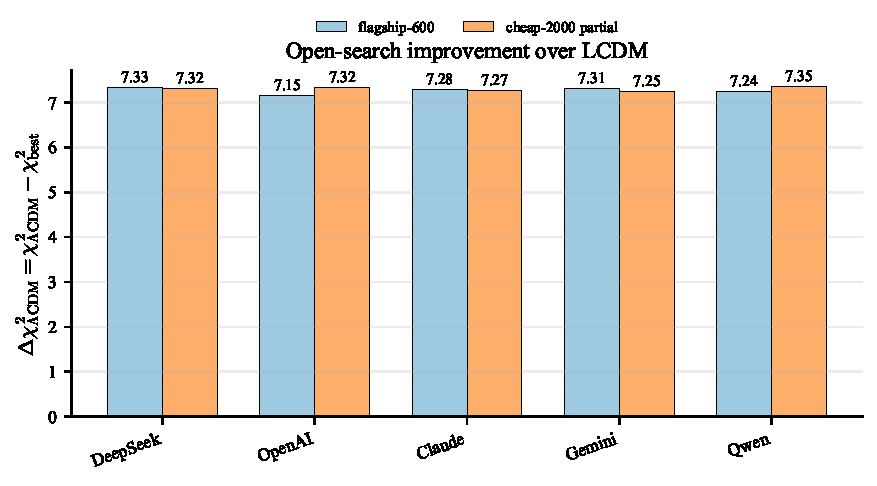
\includegraphics[width=0.82\textwidth]{figures/fig1_open_search_lcdm_improvement.pdf}
\caption{Improvement of the best open-search representative over the fixed $\Lambda$CDM reference, $\chi^2_{\Lambda{\rm CDM}}=1645.28$.  Positive values indicate lower $\chi^2$ than the reference.  The 2000-target run is censored at 72 hours, while the 600-run completed.}
\label{fig:open-lcdm-improvement}
\end{figure*}

\begin{table*}[t]
\centering
\footnotesize
\begin{ruledtabular}
\begin{tabular}{lrrrrrrr}
Model & Recorded & Open best & Open hits $<1650$ & non-EH best & non-EH hits $<2000$ & Open acc. & non-EH acc.\\
\hline
\multicolumn{8}{c}{Flagship 600-run}\\
DeepSeek V4 Pro & 600/600 & 1637.953 & 210 & 1946.871 & 3 & 0.534 & 0.070 \\
GPT-5.5 & 600/600 & 1638.130 & 80 & 1946.871 & 3 & 0.395 & 0.116 \\
Claude Opus 4.8 & 600/600 & 1637.995 & 98 & 1946.871 & 3 & 0.360 & 0.129 \\
Gemini 3.1 Pro & 600/600 & 1637.969 & 74 & 2492.845 & 0 & 0.341 & 0.103 \\
Qwen 3.7 Plus & 600/600 & 1638.035 & 29 & 1946.871 & 9 & 0.273 & 0.160 \\
\hline
\multicolumn{8}{c}{Cheap 2000-target run, censored at 72 hours}\\
DeepSeek V4 Pro & 1633/2000 & 1637.962 & 196 & 1693.860 & 27 & 0.373 & 0.164 \\
GPT-5.4 Mini & 1621/2000 & 1637.955 & 278 & 1942.427 & 12 & 0.428 & 0.124 \\
Claude Sonnet 4.6 & 1655/2000 & 1638.014 & 288 & 1946.871 & 6 & 0.372 & 0.102 \\
Gemini 2.5 Flash & 1592/2000 & 1638.034 & 276 & 1942.422 & 5 & 0.350 & 0.079 \\
Qwen 3.7 Plus & 1541/2000 & 1637.930 & 191 & 1896.001 & 3 & 0.374 & 0.144 \\
\end{tabular}
\end{ruledtabular}
\caption{Per-agent comparison by sector.  ``Recorded'' denotes recorded initial proposals over the target.  Expanded and refinement evaluations are kept in the internal memory and appendix, but they do not count toward the initial proposal target.}
\label{tab:agent-comparison}
\end{table*}

\begin{figure*}[t]
\centering
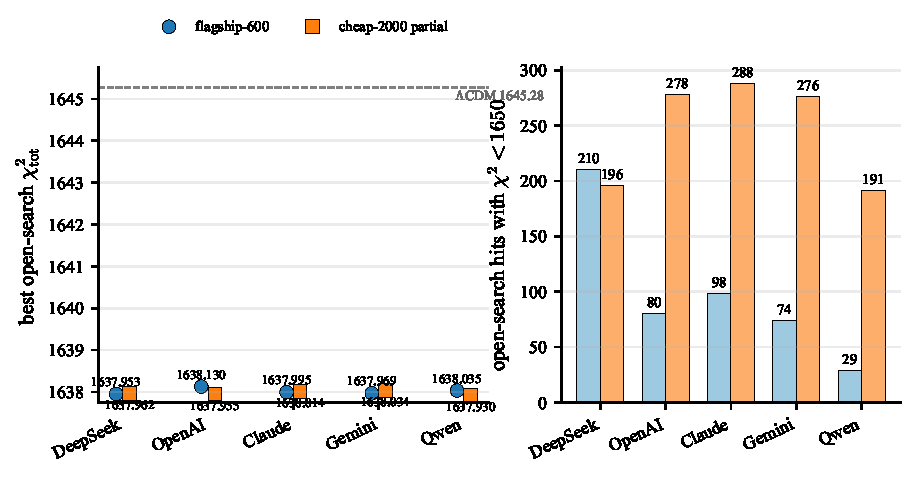
\includegraphics[width=0.95\textwidth]{figures/fig2_open_search_best_and_hits.pdf}
\caption{Open-search performance.  The left panel shows the best $\chiT$ found by each agent, with numerical values annotated.  The right panel counts accepted open-search representatives with $\chiT<1650$.  The open-search sector is already saturated: both campaigns repeatedly find the same $\chi^2\simeq1638$ basin.}
\label{fig:open-search-summary}
\end{figure*}

\begin{figure*}[t]
\centering
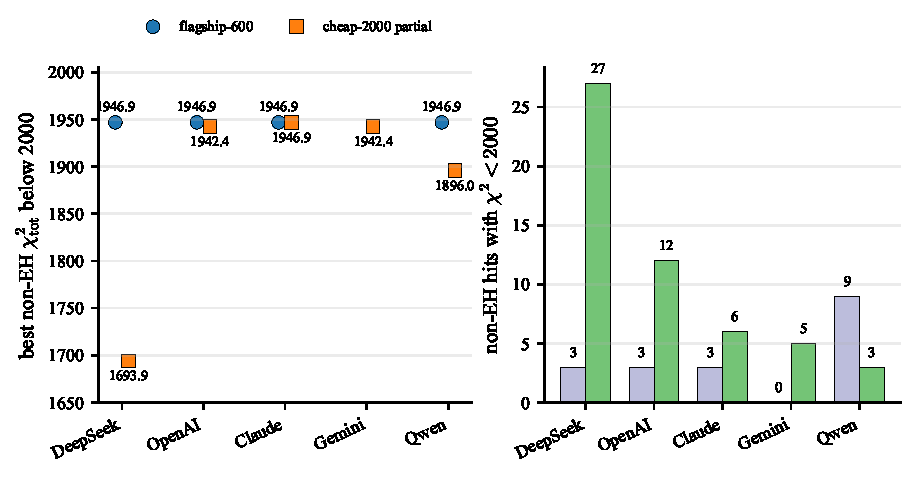
\includegraphics[width=0.95\textwidth]{figures/fig3_non_eh_best_and_hits.pdf}
\caption{New-physics sector performance.  Only non-EH representatives with $\chiT<2000$ are plotted in the left panel; agents with no such hit are left blank rather than compressing the plot with $\chi^2\simeq9434$ failures.  In the censored 2000-target run, DeepSeek finds the strongest non-EH branch, while Qwen finds a distinct $\chi^2\simeq1896$ branch.}
\label{fig:noneh-summary}
\end{figure*}

\begin{figure*}[t]
\centering
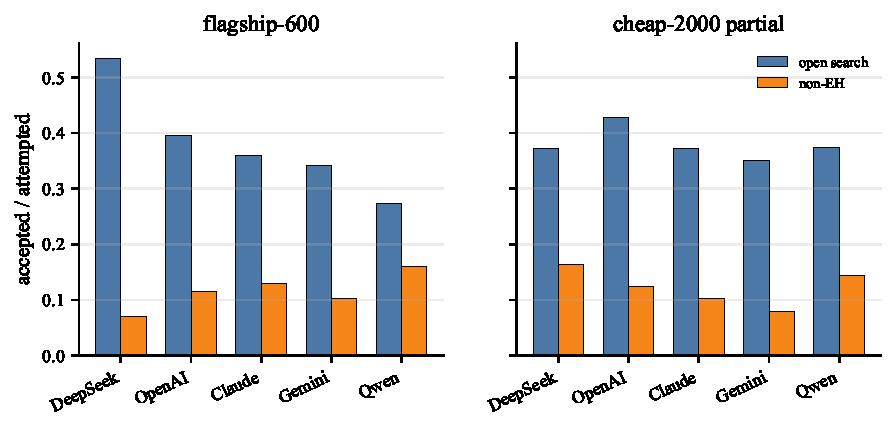
\includegraphics[width=0.88\textwidth]{figures/fig4_sector_acceptance_rates.pdf}
\caption{Acceptance rates split by proposal sector.  The non-EH sector has a consistently lower acceptance rate than open search, indicating that the difficulty is structural and not merely a lack of parameter samples.}
\label{fig:sector-acceptance}
\end{figure*}

\begin{figure}[t]
\centering
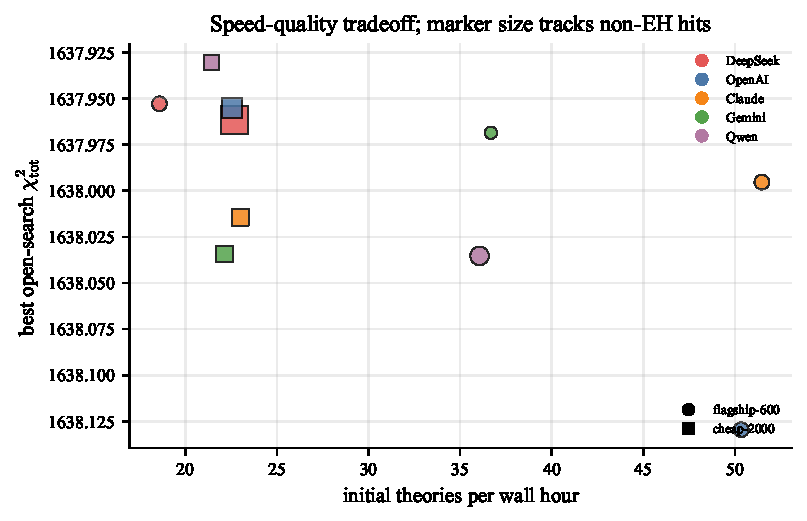
\includegraphics[width=\columnwidth]{figures/fig5_speed_quality_tradeoff.pdf}
\caption{Wall-clock efficiency versus open-search quality.  Marker size is proportional to the number of non-EH hits below $\chiT=2000$.  The fast models are not always the best new-physics explorers; DeepSeek is slower but produces the strongest non-EH signal in the censored run.}
\label{fig:speed-quality}
\end{figure}

\subsection{Open-search basin}
\label{subsec:open-results}

The open-search sector shows strong convergence across both campaigns.  Every agent reaches a representative within approximately $\Delta\chi^2\simeq7$ of the $\Lambda$CDM reference, and the best representatives cluster tightly around $\chiT\simeq1638$.  The repeated low-$\chi^2$ families are not random long operator strings: they are dominated by an Einstein--Hilbert anchor plus either a $\phi_1$ scalar sector, a two-scalar fixed sector, or weak high-curvature decorations.  Several exact operator families recur across all five cheap-run agents, including $R$ alone, $R+\phi_1^2R^2$, $R+\phi_1R_{\mu\nu\rho\sigma}R^{\mu\nu\rho\sigma}$, and two-scalar $R$ baselines.  This recurrence is evidence that the search has found a robust background expansion basin rather than a single accidental sample.

\begin{figure*}[t]
\centering
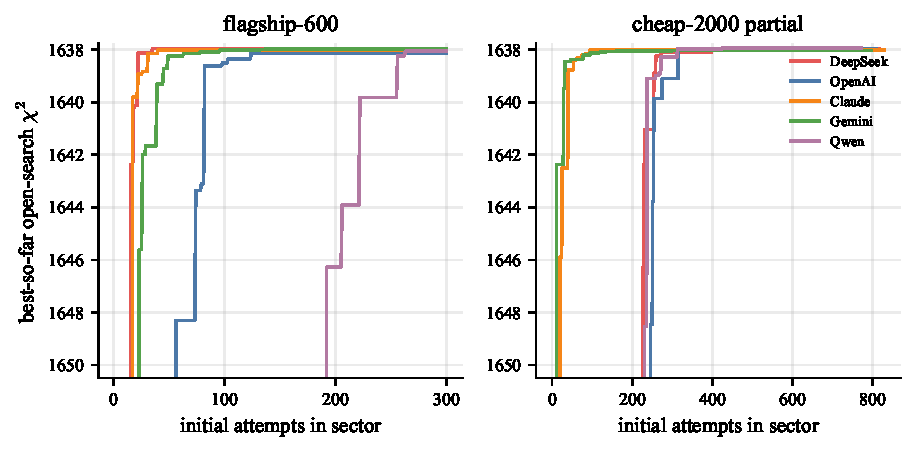
\includegraphics[width=0.95\textwidth]{figures/fig6_best_so_far_open_search.pdf}
\caption{Best-so-far open-search trajectories as a function of initial sector attempts.  The fast approach to $\chi^2\simeq1638$ explains why increasing the open-search budget from 600 to a 2000-target run gives only small gains in the global optimum.}
\label{fig:open-best-so-far}
\end{figure*}

\subsection{Non-EH new-physics search}
\label{subsec:noneh-results}

The non-EH sector behaves differently.  Its acceptance rate is lower, its median accepted $\chi^2$ is often near the poor $\chi^2\simeq9434$ plateau, and only a small fraction of accepted theories fall below $\chiT=2000$.  Nevertheless, the censored 2000-target run finds two notable non-EH branches.  DeepSeek finds a two-scalar branch with $\chiT=1693.860$, based on $\phi_2^2R$ and mixed scalar-derivative interactions.  Qwen finds a $\phi_2$-only branch with $\chiT=1896.001$ containing $\Box R$, a cubic Riemann contraction, $\phi_2^2R$, $\phi_2R_{\mu\nu}R^{\mu\nu}$, $\phi_2R_{\mu\nu\rho\sigma}R^{\mu\nu\rho\sigma}$, and derivative $\phi_2$ operators.  These are the most interesting outputs of the censored run because they are not merely EH-anchored dark-energy baselines.

\begin{figure*}[t]
\centering
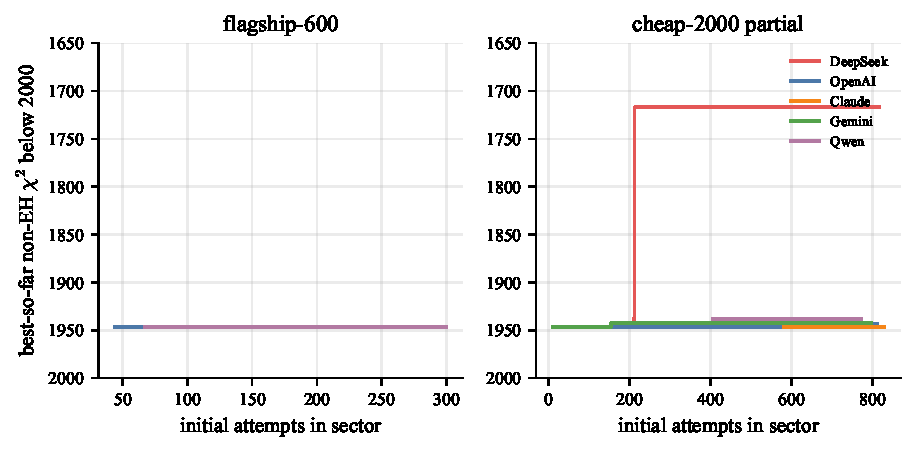
\includegraphics[width=0.95\textwidth]{figures/fig7_best_so_far_non_eh.pdf}
\caption{Best-so-far non-EH trajectories, showing only accepted representatives below $\chiT=2000$.  The blank early intervals are meaningful: many non-EH accepted branches survive the deterministic pipeline but remain far above the new-physics threshold.}
\label{fig:noneh-best-so-far}
\end{figure*}

\begin{figure}[t]
\centering
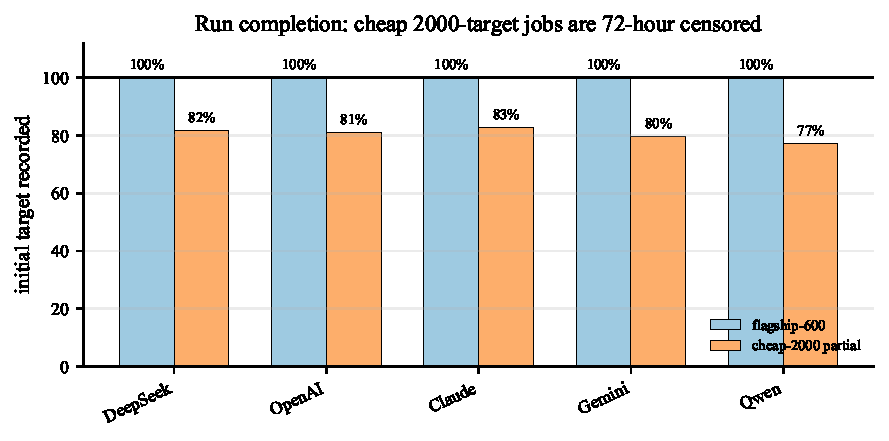
\includegraphics[width=\columnwidth]{figures/fig8_run_completion.pdf}
\caption{Completion fractions.  The 600-run finished for all agents, while the 2000-target cheap-model jobs were stopped by the 72-hour wall-time limit and should be interpreted as censored searches.}
\label{fig:completion}
\end{figure}

\section{Physical Interpretation and Limitations}
\label{sec:validation-boundaries}

The comparison clarifies the role of the autonomous agent.  For global background fitting, the agent reliably rediscovers the EH-anchored scalar basin, but this is not by itself a discovery of modified gravity.  The best open-search models often improve over the $\Lambda$CDM background reference by only $\Delta\chi^2\simeq7$, and many such models differ only in weak or effectively redundant high-curvature decorations.  Their value is mainly as a calibration of search competence.

The non-EH sector is the more relevant new-physics stress test.  The DeepSeek and Qwen branches below $\chiT=2000$ show that the search can find non-EH backgrounds substantially better than the common $\chi^2\simeq9434$ plateau.  However, they should not yet be interpreted as complete viable modified-gravity theories.  The present validation is an FLRW background validation: perturbation stability, tensor propagation, structure growth, local screening, and a full covariant degeneracy analysis remain outside the likelihood used here.

The censored 2000-target run also reveals an algorithmic lesson.  Increasing the number of proposals helps the non-EH sector more than the open-search sector, but brute force alone is inefficient.  The repeated failure of many non-EH proposals indicates that future searches should improve the non-EH proposal distribution, remove empty scalar-family pools from the scheduler, and add a more explicit diversity or motif-level prior while preserving the cold-start rule that final rankings are determined only by deterministic validation and real $\chiT$.

\section{Conclusion}
\label{sec:conclusion}

We have compared autonomous modified-gravity searches driven by five LLM proposal agents across two campaigns.  The flagship 600-run and the censored cheap 2000-target run agree on the global result: the best background fits are EH-anchored scalar sectors with $\chiT\simeq1638$.  This agreement is useful because it shows that the agent framework is robust against the choice of proposal model for the easy global optimum.

The new-physics sector remains harder and more informative.  In the censored 2000-target run, DeepSeek finds the strongest non-EH candidate, with $\chiT=1693.860$, and Qwen finds a distinct $\phi_2$-only branch at $\chiT=1896.001$.  These branches motivate follow-up studies with targeted non-EH proposal policies, perturbation-level stability checks, and additional cosmological data.  The present results should therefore be read as an autonomous background-discovery audit: the machine can efficiently locate robust expansion-history basins, but the physics pipeline must still decide which branches survive as genuine gravitational theories.

\appendix

\section{Representative Theory Archive}
\label{app:theory-archive}

This appendix records compact versions of the representative Lagrangian densities used in the discussion.  The fixed scalar pieces $\mathcal{L}_{\rm fixed}^{(i)}$ are the canonical kinetic terms plus the selected quadratic or axion potential defined in Eq.~\eqref{eq:fixed-sector}.  Only generated operators with nonzero coefficient entries in the local sample memory are displayed.  The remote run-specific Solver CSVs contain the final accepted-sample rows; when those CSVs are not present in the local archive, the numerical coefficient vector below should be read as the locally recoverable representative vector associated with the proposal memory rather than as an independent re-fit.

\begin{table*}[t]
\centering
\scriptsize
\begin{ruledtabular}
\begin{tabular}{llll}
Model & $\chiT$ & Scalar & Representative open-search content\\
\hline
DeepSeek V4 Pro & 1637.962 & phi1\_only & $R$; $R^{ab} \, R_{ab}$; $\phi_1 \, \phi_1 \, R^{ab} \, R_{ab}$ \\
GPT-5.4 Mini & 1637.955 & both & $R$; $R^{cd}_{ab} \, R^{afh}_{c} \, R^{b}_{fdh}$ \\
Claude Sonnet 4.6 & 1638.014 & both & $R$; $\phi_2 \, R \, R$; $\phi_2 \, \phi_2 \, \phi_2 \, \phi_2 \, \phi_2$ \\
Gemini 2.5 Flash & 1638.034 & phi1\_only & $R$; $R^{bd}_{ac} \, R^{agh}_{b} \, R^{c}_{dgh}$ \\
Qwen 3.7 Plus & 1637.930 & phi1\_only & $R$; $\phi_1 \, R^{bcd}_{a} \, R^{a}_{bcd}$; $\phi_1 \, \phi_1 \, R^{bcd}_{a} \, R^{a}_{bcd}$ \\
\end{tabular}
\end{ruledtabular}
\caption{Best open-search representative for each cheap-run agent.  Full coefficient-substituted densities for the most useful representatives are written below.}
\label{tab:appendix-open-best}
\end{table*}

\begin{table*}[t]
\centering
\scriptsize
\begin{ruledtabular}
\begin{tabular}{llll}
Model & $\chiT$ & Scalar & Representative non-EH content\\
\hline
DeepSeek V4 Pro & 1693.860 & both & $\phi_2 \, \phi_2 \, R$; $\phi_1 \, \Box \phi_1 \, \phi_2$; $\phi_1 \, \Box \phi_1 \, \phi_2 \, \phi_2$ \\
GPT-5.4 Mini & 1942.427 & phi2\_only & $R^{bcd}_{a} \, R^{a}_{bcd}$; $\Box R \, R^{c}_{c}$; $\phi_2 \, \phi_2 \, R$; $+3$ more \\
Claude Sonnet 4.6 & 1946.871 & phi2\_only & $R \, R^{ab} \, R_{ab}$; $R_{ab} \, R^{adef} \, R^{b}_{def}$; $\phi_2 \, \phi_2 \, R^{ab} \, R_{ab}$; $+5$ more \\
Gemini 2.5 Flash & 1942.422 & phi2\_only & $R^{bcd}_{a} \, R^{a}_{bcd}$; $\phi_2 \, R$; $\phi_2 \, R^{ab} \, R_{ab}$; $+1$ more \\
Qwen 3.7 Plus & 1896.001 & phi2\_only & $\Box R$; $R^{cd}_{ab} \, R^{afh}_{c} \, R^{b}_{fdh}$; $\phi_2 \, \phi_2 \, R$; $+5$ more \\
\end{tabular}
\end{ruledtabular}
\caption{Best non-EH representative for each cheap-run agent.  Rows with $\chiT\simeq9434$ are retained as diagnostics but are not expanded into long equations unless they pass the $\chiT<2000$ new-physics threshold.}
\label{tab:appendix-noneh-best}
\end{table*}

\begin{table*}[t]
\centering
\scriptsize
\begin{ruledtabular}
\begin{tabular}{llll}
Scalar sector & Best $\chiT$ & Agents finding family & Repeated operator content\\
\hline
phi1\_only & 1637.930 & Claude, DeepSeek, Gemini, OpenAI, Qwen & $R$; $\phi_1 \, \phi_1 \, R \, R$ \\
phi1\_only & 1637.930 & Claude, DeepSeek, Gemini, OpenAI, Qwen & $R$; $\phi_1 \, R^{bcd}_{a} \, R^{a}_{bcd}$ \\
phi1\_only & 1637.937 & Claude, DeepSeek, Gemini, OpenAI, Qwen & $R$ \\
both & 1637.950 & Claude, DeepSeek, Gemini, OpenAI, Qwen & $R$ \\
phi2\_only & 1946.871 & DeepSeek, OpenAI & $\phi_2 \, R^{ab} \, R_{ab}$; $\phi_2 \, R^{bcd}_{a} \, R^{a}_{bcd}$ \\
\end{tabular}
\end{ruledtabular}
\caption{Repeated low-$\chi^2$ families in the censored cheap 2000-target run.  Exact-family repetition across agents is a stronger signal than a single isolated low-$\chi^2$ proposal.}
\label{tab:appendix-repeated}
\end{table*}

\begin{widetext}

\paragraph*{DeepSeek V4 Pro, non-EH, $\chi^2=1693.860$.}
\begin{equation}
\begin{split}
\mathscr{L}_{A1}
=\sqrt{-g}\left\{\Mp^2\left[\alpha\,\Lambda^{-2}\,\phi_2 \, \phi_2 \, R + \beta\,\Lambda^{-1}\,\phi_1 \, \Box \phi_1 \, \phi_2 + \gamma\,\Lambda^{-2}\,\phi_1 \, \Box \phi_1 \, \phi_2 \, \phi_2\right] + \mathcal{L}_{\rm fixed}^{(1)} + \mathcal{L}_{\rm fixed}^{(2)}\right\}.
\end{split}
\end{equation}
Available nonzero generated-coefficient vector from local sample memory:
\begin{equation}
\alpha=-7251,\; \beta=-57.47,\; \gamma=3.64\times10^{11}.
\end{equation}
Representative background sample:
\begin{equation}
H_0=66.3,\; \Omega_{m0}=0.3368,\; \lambda_H=1.01\times10^{4}.
\end{equation}


\paragraph*{GPT-5.4 Mini, non-EH, $\chi^2=1942.427$.}
\begin{equation}
\begin{split}
\mathscr{L}_{A2}
=\sqrt{-g}\left\{\Mp^2\left[\alpha\,\Lambda^{-2}\,R^{bcd}_{a} \, R^{a}_{bcd} + \beta\,\Lambda^{-4}\,\Box R \, R^{c}_{c} + \gamma\,\Lambda^{-2}\,\phi_2 \, \phi_2 \, R + \delta\,\Lambda^{-4}\,\phi_2 \, \phi_2 \, R^{ab} \, R_{ab} + \epsilon\,\Lambda^{-4}\,\phi_2 \, \phi_2 \, R^{bcd}_{a} \, R^{a}_{bcd} + \zeta\,\nabla^{a}\phi_2 \, \nabla_{a}\phi_2\right] + \mathcal{L}_{\rm fixed}^{(2)}\right\}.
\end{split}
\end{equation}
Available nonzero generated-coefficient vector from local sample memory:
\begin{equation}
\alpha=-23.52,\; \beta=-2.89\times10^{8},\; \gamma=1.44\times10^{-4},\; \delta=-1185,\; \epsilon=5503,\; \zeta=1.21\times10^{6}.
\end{equation}
Representative background sample:
\begin{equation}
H_0=58,\; \Omega_{m0}=0.2839,\; \lambda_H=1957.
\end{equation}


\paragraph*{Claude Sonnet 4.6, non-EH, $\chi^2=1946.871$.}
\begin{equation}
\begin{split}
\mathscr{L}_{A3}
=\sqrt{-g}\left\{\Mp^2\left[\alpha\,\Lambda^{-4}\,R \, R^{ab} \, R_{ab} + \beta\,\Lambda^{-4}\,R_{ab} \, R^{adef} \, R^{b}_{def} + \gamma\,\Lambda^{-4}\,\phi_2 \, \phi_2 \, R^{ab} \, R_{ab} + \delta\,\Lambda^{-4}\,\phi_2 \, \phi_2 \, R^{bcd}_{a} \, R^{a}_{bcd} + \epsilon\,\Lambda^{2}\,\phi_2 \, \phi_2 + \zeta\,\phi_2 \, \Box \phi_2 + \eta\,\Lambda^{-1}\,\phi_2 \, \phi_2 \, \phi_2 \, \phi_2 \, \phi_2 + \theta\,\Lambda^{-2}\,\phi_2 \, \phi_2 \, \phi_2 \, \phi_2 \, \phi_2 \, \phi_2\right] + \mathcal{L}_{\rm fixed}^{(2)}\right\}.
\end{split}
\end{equation}
Available nonzero generated-coefficient vector from local sample memory:
\begin{equation}
\alpha=1.64\times10^{-10},\; \beta=0.1381,\; \gamma=2.83\times10^{16},\; \delta=6.19\times10^{13},\; \epsilon=-2.239,\; \zeta=-0.03945,\; \eta=-1.18\times10^{12},\; \theta=5.53\times10^{-4}.
\end{equation}
Representative background sample:
\begin{equation}
H_0=60.25,\; \Omega_{m0}=0.3142,\; \lambda_H=5371.
\end{equation}


\paragraph*{Gemini 2.5 Flash, non-EH, $\chi^2=1942.422$.}
\begin{equation}
\begin{split}
\mathscr{L}_{A4}
=\sqrt{-g}\left\{\Mp^2\left[\alpha\,\Lambda^{-2}\,R^{bcd}_{a} \, R^{a}_{bcd} + \beta\,\Lambda^{-1}\,\phi_2 \, R + \gamma\,\Lambda^{-3}\,\phi_2 \, R^{ab} \, R_{ab} + \delta\,\Lambda^{-3}\,\phi_2 \, R^{bcd}_{a} \, R^{a}_{bcd}\right] + \mathcal{L}_{\rm fixed}^{(2)}\right\}.
\end{split}
\end{equation}
Available nonzero generated-coefficient vector from local sample memory:
\begin{equation}
\alpha=-590.8,\; \beta=0.2832,\; \gamma=3.58\times10^{7},\; \delta=3.63\times10^{8}.
\end{equation}
Representative background sample:
\begin{equation}
H_0=62.61,\; \Omega_{m0}=0.2867,\; \lambda_H=1.11\times10^{4}.
\end{equation}


\paragraph*{Qwen 3.7 Plus, non-EH, $\chi^2=1896.001$.}
\begin{equation}
\begin{split}
\mathscr{L}_{A5}
=\sqrt{-g}\left\{\Mp^2\left[\alpha\,\Lambda^{-2}\,\Box R + \beta\,\Lambda^{-4}\,R^{cd}_{ab} \, R^{afh}_{c} \, R^{b}_{fdh} + \gamma\,\Lambda^{-2}\,\phi_2 \, \phi_2 \, R + \delta\,\Lambda^{-3}\,\phi_2 \, R^{ab} \, R_{ab} + \epsilon\,\Lambda^{-3}\,\phi_2 \, R^{bcd}_{a} \, R^{a}_{bcd} + \zeta\,\Lambda^{-4}\,\phi_2 \, \Box \phi_2 \, R + \eta\,\phi_2 \, \Box \phi_2 + \theta\,\Lambda^{-2}\,\phi_2 \, \phi_2 \, \nabla^{a}\phi_2 \, \nabla_{a}\phi_2\right] + \mathcal{L}_{\rm fixed}^{(2)}\right\}.
\end{split}
\end{equation}
Available nonzero generated-coefficient vector from local sample memory:
\begin{equation}
\alpha=4.56\times10^{9},\; \beta=-1.53\times10^{6},\; \gamma=-2.09\times10^{-4},\; \delta=8.25\times10^{18},\; \epsilon=-3.34\times10^{6},\; \zeta=3.31\times10^{9},\; \eta=1.68\times10^{6},\; \theta=-9.04\times10^{16}.
\end{equation}
Representative background sample:
\begin{equation}
H_0=62.32,\; \Omega_{m0}=0.2641,\; \lambda_H=2.3\times10^{4}.
\end{equation}


\paragraph*{DeepSeek V4 Pro, open search, $\chi^2=1637.962$.}
\begin{equation}
\begin{split}
\mathscr{L}_{A6}
=\sqrt{-g}\left\{\Mp^2\left[\alpha\,R + \beta\,\Lambda^{-2}\,R^{ab} \, R_{ab} + \gamma\,\Lambda^{-4}\,\phi_1 \, \phi_1 \, R^{ab} \, R_{ab}\right] + \mathcal{L}_{\rm fixed}^{(1)}\right\}.
\end{split}
\end{equation}
Available nonzero generated-coefficient vector from local sample memory:
\begin{equation}
\alpha=0.5,\; \beta=-9134,\; \gamma=-7.01\times10^{8}.
\end{equation}
Representative background sample:
\begin{equation}
H_0=65.41,\; \Omega_{m0}=0.3025,\; \lambda_H=2244.
\end{equation}


\paragraph*{GPT-5.4 Mini, open search, $\chi^2=1637.955$.}
\begin{equation}
\begin{split}
\mathscr{L}_{A7}
=\sqrt{-g}\left\{\Mp^2\left[\alpha\,R + \beta\,\Lambda^{-4}\,R^{cd}_{ab} \, R^{afh}_{c} \, R^{b}_{fdh}\right] + \mathcal{L}_{\rm fixed}^{(1)} + \mathcal{L}_{\rm fixed}^{(2)}\right\}.
\end{split}
\end{equation}
Available nonzero generated-coefficient vector from local sample memory:
\begin{equation}
\alpha=0.5,\; \beta=3.82\times10^{9}.
\end{equation}
Representative background sample:
\begin{equation}
H_0=68.17,\; \Omega_{m0}=0.2735,\; \lambda_H=4076.
\end{equation}


\paragraph*{Claude Sonnet 4.6, open search, $\chi^2=1638.014$.}
\begin{equation}
\begin{split}
\mathscr{L}_{A8}
=\sqrt{-g}\left\{\Mp^2\left[\alpha\,R + \beta\,\Lambda^{-3}\,\phi_2 \, R \, R + \gamma\,\Lambda^{-1}\,\phi_2 \, \phi_2 \, \phi_2 \, \phi_2 \, \phi_2\right] + \mathcal{L}_{\rm fixed}^{(1)} + \mathcal{L}_{\rm fixed}^{(2)}\right\}.
\end{split}
\end{equation}
Available nonzero generated-coefficient vector from local sample memory:
\begin{equation}
\alpha=0.5,\; \beta=3.16\times10^{9},\; \gamma=-1\times10^{5}.
\end{equation}
Representative background sample:
\begin{equation}
H_0=70.8,\; \Omega_{m0}=0.3009,\; \lambda_H=3102.
\end{equation}


\paragraph*{Gemini 2.5 Flash, open search, $\chi^2=1638.034$.}
\begin{equation}
\begin{split}
\mathscr{L}_{A9}
=\sqrt{-g}\left\{\Mp^2\left[\alpha\,R + \beta\,\Lambda^{-4}\,R^{bd}_{ac} \, R^{agh}_{b} \, R^{c}_{dgh}\right] + \mathcal{L}_{\rm fixed}^{(1)}\right\}.
\end{split}
\end{equation}
Available nonzero generated-coefficient vector from local sample memory:
\begin{equation}
\alpha=0.5,\; \beta=2.98\times10^{12}.
\end{equation}
Representative background sample:
\begin{equation}
H_0=68.77,\; \Omega_{m0}=0.3011,\; \lambda_H=1.3\times10^{4}.
\end{equation}


\paragraph*{Qwen 3.7 Plus, open search, $\chi^2=1637.930$.}
\begin{equation}
\begin{split}
\mathscr{L}_{A10}
=\sqrt{-g}\left\{\Mp^2\left[\alpha\,R + \beta\,\Lambda^{-3}\,\phi_1 \, R^{bcd}_{a} \, R^{a}_{bcd} + \gamma\,\Lambda^{-4}\,\phi_1 \, \phi_1 \, R^{bcd}_{a} \, R^{a}_{bcd}\right] + \mathcal{L}_{\rm fixed}^{(1)}\right\}.
\end{split}
\end{equation}
Available nonzero generated-coefficient vector from local sample memory:
\begin{equation}
\alpha=0.5,\; \beta=-4.67\times10^{13},\; \gamma=9.69\times10^{14}.
\end{equation}
Representative background sample:
\begin{equation}
H_0=61.73,\; \Omega_{m0}=0.2844,\; \lambda_H=1.88\times10^{4}.
\end{equation}

\end{widetext}

\bibliographystyle{apsrev4-2}
\bibliography{main2}

\end{document}
